%% solar_nbhood.tex

Even within the Milky Way, measuring velocities and distances was and still is a
complicated endeavour.  Earth is revolving around our Sun, and the Solar System
is orbiting around the Galactic center, which means relative motions have to be
carefully examined.  From some locations on Earth, a dense strip of starlight is
visible across the night sky which is indicative of the Galaxy's disk structure.

\begin{figure}[h]
    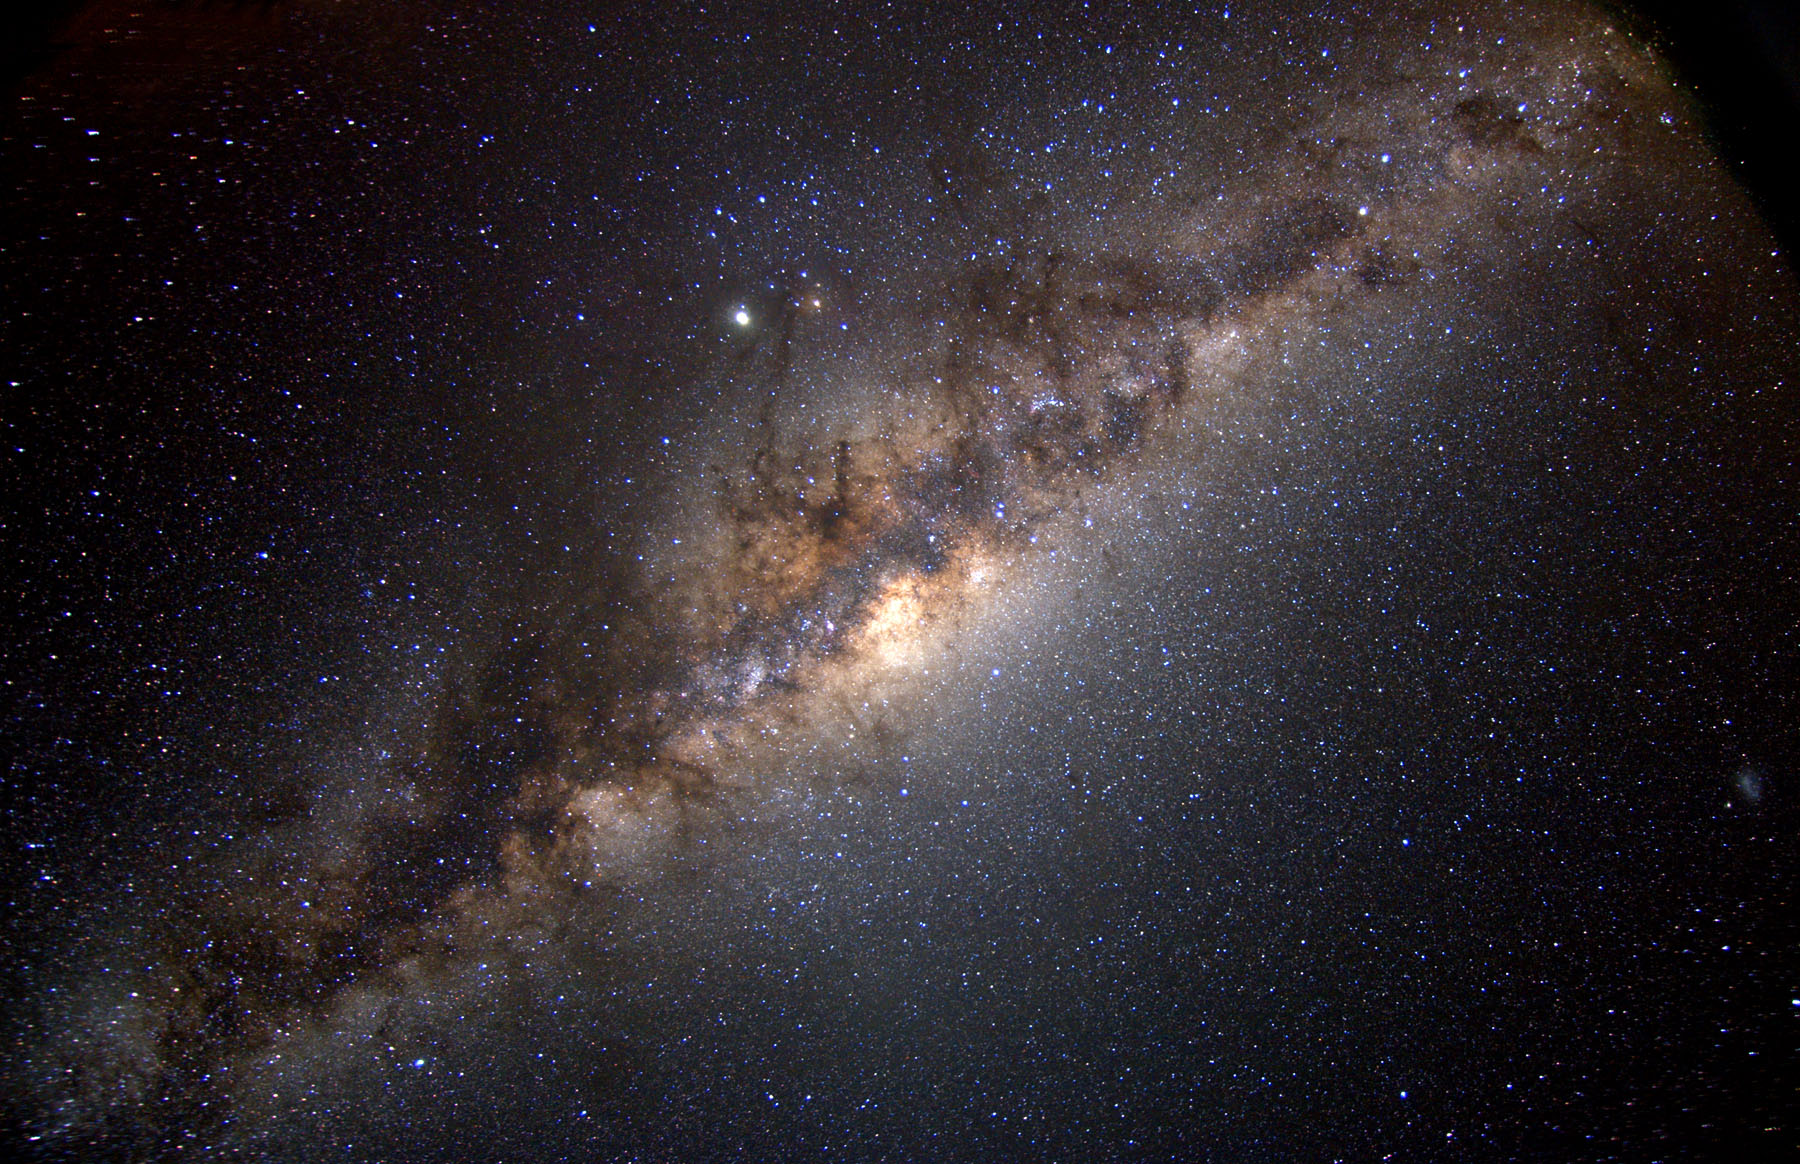
\includegraphics{apod080104}
    \caption[The Milky Way: APOD 2008 January
    4]{\href{https://apod.nasa.gov/apod/ap080104.html}{APOD 2008 January 4}: The
    Milky Way at 5000 meters.\\
    View on our own galaxy from within (recorded in the Chilean Andes).  The
    band of the dense collection of stars from the disk and the Galactic center
    is partially covered by the typical extinction features due to dust
    clouds.  This suggest that the Milky Way possesses a stellar disk.\\
    \textit{Credit \& Copyright: Serge Brunier}}
    \figlbl{milkyway}
\end{figure}

From far away it is quite easy to recognize the typical morphology of other
galaxies through direct observations\sidenote{Provided the telescope has enough
angular resolution.}.  Measuring their rotational properties already becomes
increasingly difficult, deducing the shape and rotation patterns of the Milky
Way from within however is an undertaking of its own.

A possibly random and dense distribution of stars as it appears in galaxies
should in principle collapse towards its potential well.  Like in many other
astrophysical scenarii, pressure gradients can take a stabilizing role and
balance gravity.  These balancing pressures depend on different physical
processes and generally define limiting scales.  For some galaxies, e.g.
ellipticals, the stars' random motions are the dominant drivers towards
stability, for spiral galaxies it is their rotation about the disk's center.  In
contrast to orbiting systems such as the Sun and Earth, where most of the mass
is located near the guiding center of the orbits, the Milky Way's mass
distribution is more complex with different elements such as various forms of
hydrogen gas, dust, stars, and stellar remnants.  In general, the study of
galactic rotation through stars can yield insights not only into the galaxy's
morphology, but also into its formation history and mass composition.  One of
the most powerful tools therefor is the rotation curve $V(R)$.  It characterizes
the orbital velocity as a function of distance from the Galactic center. By
measuring how $V(R)$ behaves with radius, we can draw conclusions about the
Milky Way's size, total mass, and the distribution thereof.  A solid-body
rotation $V \propto R$ would mean that the enclosed mass ideally increases with
$R^{2}$, Keplerian orbits go as $V \propto R^{-\half}$, whereas $V \propto
\text{const.}$ is a result of the enclosed mass increasing as $R$.

Milky Way's rotation curve can be probed through its stars. Prime observable is
the radial velocity $v_{r}$, and in principle the tangential velocity $v_{t}$,
distance from Earth $d$ and longitude on the sky $l$ too.  Measurements of these
quantities can be combined to the so-called \textit{Oort's constants}
\begin{align}
    &A = \frac{v_{r}}{d\sin{2l}} \hspace{0.5cm}\nonumber\\[5pt]%
    &B = \frac{v_{t}}{d} - A\cos{2l}.
    \eqlbl{obs_oortsC}
\end{align}

A caveat is the assumption that the stars, including the Sun, are on circular
orbits, which is only approximately true.  Moreover, it assumes the Milky Way
has a monotonically decreasing, symmetric potential.  Again, this is not
entirely true as spiral arms can introduce over-densities which manifest as
asymmetries and locally break monotonic behaviour in the potential.  Still,
within their limits the Oort's constants are very useful, because they can be
rewritten as
\begin{align}
    &A = -\frac{1}{2} \left[\frac{\derivd V}{\derivd R} - \frac{V_{0}}{R_{0}}\right]\nonumber\\[5pt]%
    &B = -\frac{1}{2}\left[\frac{V_{0}}{R_{0}} + \frac{\derivd V}{\derivd R}\right].
    \eqlbl{oortsC}
\end{align}

These constants express the shear and vorticity of the disk in the solar
neighbourhood.  The shear essentially measures a deviation from solid-body
rotation, the vorticity how the angular momentum varies with small changes in
radius.  Adding both $A+B = -\frac{\derivd V}{\derivd R}$